% !TEX program = pdflatex
% ----------------------------------------------------------------------------------------
% Thermally induced deformation and conjugate heat transfer in a channel with a thermoelastic
% wall.  Manuscript for the International Journal of Numerical Methods for Heat & Fluid Flow.
% Build:  pdflatex main && bibtex main && pdflatex main && pdflatex main
% All computed numbers are macros from numbers.tex, generated by code/make_numbers.py.
% ----------------------------------------------------------------------------------------
\documentclass[11pt,a4paper]{article}

\usepackage[a4paper,margin=2.5cm]{geometry}
\usepackage[T1]{fontenc}
\usepackage{mathptmx}            % Times-compatible text and maths
\usepackage{amsmath,amssymb,bm}
\usepackage{booktabs,array}
\usepackage{siunitx}
\sisetup{detect-all=true,per-mode=symbol,exponent-product=\times}
\usepackage{graphicx}
\usepackage{xcolor}
\usepackage{enumitem}
\usepackage{microtype}
\usepackage[round,authoryear,comma]{natbib}
\usepackage{caption}
\captionsetup{labelfont=bf,labelsep=period,font=small,justification=raggedright,singlelinecheck=false}
\usepackage{titlesec}
% Emerald headings: first level bold, lower levels medium italic
\titleformat{\section}{\normalfont\large\bfseries}{\thesection.}{0.6em}{}
\titleformat{\subsection}{\normalfont\itshape}{\thesubsection}{0.6em}{}
\titleformat{\subsubsection}{\normalfont\itshape}{\thesubsubsection}{0.6em}{}
\titlespacing*{\section}{0pt}{1.6ex plus .4ex}{1ex}
\titlespacing*{\subsection}{0pt}{1.3ex plus .3ex}{0.7ex}
\providecommand{\doi}[1]{doi:~\href{https://doi.org/#1}{#1}}
\usepackage[hidelinks,pdftitle={Thermally induced deformation and conjugate heat transfer in a channel with a thermoelastic wall},pdfkeywords={conjugate heat transfer; thermoelasticity; fluid--structure interaction; finite element method; flexible channel wall; thermal bending}]{hyperref}

\renewcommand{\thetable}{\Roman{table}}      % Emerald: tables in Roman numerals
\linespread{1.12}
\setlength{\parskip}{0pt}
\setlength{\parindent}{1.2em}
\setlist{nosep,leftmargin=1.6em}

% AUTO-GENERATED by code/make_numbers.py -- do not edit by hand.

\newcommand{\NumRe}{50}
\newcommand{\NumPr}{6.97}
\newcommand{\NumPe}{348}
\newcommand{\NumDp}{72}
\newcommand{\NumTauW}{0.6}
\newcommand{\NumRi}{1.7\times10^{-3}}
\newcommand{\NumBr}{1.0\times10^{-6}}
\newcommand{\NumDTstar}{4.17}
\newcommand{\NumDTt}{60}
\newcommand{\NumDTb}{1.44}
\newcommand{\NumQoverH}{1.55}
\newcommand{\NumHrigid}{3231}
\newcommand{\NumThetaBar}{32.3}
\newcommand{\NumKappa}{1.4}
\newcommand{\NumDs}{9.64}
\newcommand{\NumNtheta}{2.90\times10^{4}}
\newcommand{\NumNcr}{1.06\times10^{5}}
\newcommand{\NumNratio}{0.275}
\newcommand{\NumTcr}{117}
\newcommand{\NumMb}{3.64}
\newcommand{\NumMuL}{1.65}
\newcommand{\NumWlin}{1.57\times10^{-4}}
\newcommand{\NumWlinH}{0.315}
\newcommand{\NumWfrozen}{2.19\times10^{-4}}
\newcommand{\NumWfrozenH}{0.438}
\newcommand{\NumWsc}{2.14\times10^{-4}}
\newcommand{\NumWscH}{0.428}
\newcommand{\NumAmpFrozen}{1.39}
\newcommand{\NumAmpSc}{1.36}
\newcommand{\NumAmpEuler}{1.38}
\newcommand{\NumRelax}{5.9}
\newcommand{\NumExcessFrozen}{2.3}
\newcommand{\NumHmidFrozen}{1.4377}
\newcommand{\NumHmidSc}{1.428}
\newcommand{\NumHmidMm}{0.719}
\newcommand{\NumWfrozenMm}{0.219}
\newcommand{\NumSlope}{0.028}
\newcommand{\NumArcStrain}{1.39\times10^{-4}}
\newcommand{\NumFibreStrain}{9.89\times10^{-4}}
\newcommand{\NumSigBend}{4.2}
\newcommand{\NumSigMemb}{9.7}
\newcommand{\NumSigMax}{13.9}
\newcommand{\NumSigFrac}{0.15}
\newcommand{\NumMmid}{6.4}
\newcommand{\NumPbar}{84}
\newcommand{\NumPentry}{120}
\newcommand{\NumPexit}{48}
\newcommand{\NumWp}{9.19\times10^{-8}}
\newcommand{\NumWpBC}{1.27\times10^{-7}}
\newcommand{\NumGammaLin}{1714.3}
\newcommand{\NumGammaLinRound}{1714}
\newcommand{\NumGammaBC}{1726.3}
\newcommand{\NumGammaBCRound}{1726}
\newcommand{\NumGammaMixed}{2382.1}
\newcommand{\NumDpLub}{36}
\newcommand{\NumDpLubRatio}{0.50}
\newcommand{\NumDpLubDrop}{50}
\newcommand{\NumHydFeedbackPct}{0.06}
\newcommand{\NumExcessRatio}{1.29}
\newcommand{\NumExcessDeformed}{1.99}
\newcommand{\NumReHL}{0.42}
\newcommand{\NumLoverLT}{1.7}
\newcommand{\NumLT}{17.4}
\newcommand{\NumFeedbackExtraK}{0.45}
\newcommand{\NumFeedbackPct}{0.5}
\newcommand{\NumQw}{5.5}
\newcommand{\NumQs}{6.0}
\newcommand{\NumQb}{9.1}
\newcommand{\NumExcessW}{3.0}
\newcommand{\NumExcessS}{3.9}
\newcommand{\NumExcessB}{17}
\newcommand{\NumRatioW}{0.30}
\newcommand{\NumRatioS}{0.33}
\newcommand{\NumWHs}{0.56}
\newcommand{\NumWHb}{1.16}
\newcommand{\NumStainlessKappa}{6.9\times10^{-3}}
\newcommand{\NumStainlessWH}{1.6\times10^{-3}}
\newcommand{\NumPolymerOverStainless}{203}
\newcommand{\QPointMin}{1.00000}
\newcommand{\QPointMax}{1.00000}
\newcommand{\QPatchMax}{5\times10^{-13}}
\newcommand{\QPinCoarse}{0.9999}
\newcommand{\QPinTwo}{0.99793}
\newcommand{\QPinFour}{0.99800}
\newcommand{\QPinEight}{0.99800}
\newcommand{\QPinDefect}{0.20}
\newcommand{\QPinAxialLast}{3\times10^{-8}}
\newcommand{\QPinThickLast}{4\times10^{-6}}
\newcommand{\QPinThickFirst}{6.2\times10^{-5}}
\newcommand{\QClampLastTwo}{-0.0195}
\newcommand{\QClampOrderTwo}{1.7}
\newcommand{\QClampInfTwo}{-0.0192}
\newcommand{\QClampGCITwo}{2.0}
\newcommand{\QClampLastFour}{-0.0180}
\newcommand{\QClampOrderFour}{1.3}
\newcommand{\QClampInfFour}{-0.0175}
\newcommand{\QClampGCIFour}{3.8}
\newcommand{\QClampLastEight}{-0.0174}
\newcommand{\QClampOrderEight}{1.1}
\newcommand{\QClampInfEight}{-0.0168}
\newcommand{\QClampGCIEight}{4.2}
\newcommand{\QClampCoarse}{-0.080}
\newcommand{\QClampTwelveTwo}{-0.045}
\newcommand{\QElemMax}{1536}
\newcommand{\NLwFE}{2.221\times10^{-4}}
\newcommand{\NLwFEH}{0.444}
\newcommand{\NLlinRatio}{0.9980}
\newcommand{\NLampFE}{1.413}
\newcommand{\NLoverSc}{1.038}
\newcommand{\NLoverScPct}{3.8}
\newcommand{\NLoverFrozenPct}{1.5}
\newcommand{\NLNmidLin}{29.67}
\newcommand{\NLNmidNL}{27.73}
\newcommand{\NLNmidLinPct}{2.2}
\newcommand{\NLNmidNLPct}{1.5}
\newcommand{\NLrelaxFE}{6.5}
\newcommand{\NLconvAxial}{0.014}
\newcommand{\NLconvThick}{0.07}
\newcommand{\NLtangentMax}{2\times10^{-5}}
\newcommand{\NLnewtonMax}{5}
\newcommand{\NLresMax}{4\times10^{-11}}
\newcommand{\NLthetaBar}{32.3}
\newcommand{\NLNmidAmpEuler}{1.355}
\newcommand{\IndElements}{3072}
\newcommand{\IndW}{2.222\times10^{-4}}
\newcommand{\IndDiffPct}{0.018}
\newcommand{\IndLinDiffPct}{0.0000}
\newcommand{\IndNDiffPct}{0.01}
\newcommand{\IndConv}{0.03}
\newcommand{\SlForceRatio}{0.275}
\newcommand{\SlFirstPct}{3.8}
\newcommand{\SlLastPct}{-0.2}
\newcommand{\SlLastDL}{0.025}
\newcommand{\SlLastFrozenPct}{20}
\newcommand{\SlMidPct}{0.9}
\newcommand{\SlMeshPct}{0.01}
\newcommand{\SlMidDL}{0.050}
                              % generated: every computed value used in the text

% ---- notation shortcuts ----
\newcommand{\bn}{\bm{n}}
\newcommand{\bu}{\bm{u}}
\newcommand{\bd}{\bm{d}}
\newcommand{\bsig}{\bm{\sigma}}
\newcommand{\beps}{\bm{\varepsilon}}
\newcommand{\bI}{\bm{I}}
\newcommand{\bphi}{\bm{\varphi}}
\newcommand{\bv}{\bm{v}}
\newcommand{\bD}{\bm{D}}
\newcommand{\bwhat}{\widehat{\bm{w}}}
\newcommand{\Om}{\Omega}
\newcommand{\Ga}{\Gamma}
\newcommand{\dd}{\mathrm{d}}
\newcommand{\qpp}{q^{\prime\prime}}
\newcommand{\ncr}{N_{\mathrm{cr}}}
\newcommand{\kth}{\kappa_{\mathrm{th}}}
\newcommand{\Nc}{N_c}
\newcommand{\wmax}{w_{\max}}

\title{\bfseries Thermally induced deformation and conjugate heat transfer in a channel with a
thermoelastic wall: formulation, reduced-order analysis and finite-element verification}
\author{}
\date{}

\begin{document}
\maketitle
\vspace{-2.2em}

\begin{abstract}\noindent
\textbf{Purpose} -- To formulate, analyse and partly verify a conjugate heat-transfer problem in which a thin
polymer strip, heated on its outer face, forms one wall of a laminar slit channel and bows because of through-wall
thermal expansion, widening the passage.\\
\textbf{Design/methodology/approach} -- A steady formulation with one consistent set of sign and interface
conventions is given. Closed-form thermoelastic results (free curvature, bowing, buckling, beam--column
amplification) define a baseline and admissibility guards. A finite-element method and a
fixed-point coupling algorithm are specified; the wall is verified with two independent plane-strain codes, including a restrained,
geometrically nonlinear case.\\
\textbf{Findings} -- For water at $\mathrm{Re}=\NumRe$ and a flux of \SI{5}{\kilo\watt\per\square\metre} on a
\SI{3}{\milli\metre} PEEK-class strip, the strip bows away from the channel by $\NumWscH\,H_0$
(reduced order) or $\NLwFEH\,H_0$ (finite element); the difference of $\NLoverScPct\,\%$ vanishes for slender strips. Deformation and stress,
not buckling, bound the flux. Indicative estimates suggest a roughly halved pressure drop and a higher wall excess
temperature, while the return effect of the flow on the bow is small.\\
\textbf{Research limitations/implications} -- No coupled fluid--structure result is reported; the flow-side
estimates are reduced-order, the material data are representative; contact, heater and casing are idealised.\\
\textbf{Originality/value} -- Thermally driven wall deformation in forced convection, a verified wall model and a specified, not yet executed, coupled solver.\\[0.5ex]
\textbf{Keywords} Conjugate heat transfer, Thermoelasticity, Fluid--structure interaction, Finite element method,
Flexible channel wall, Thermal bending\\
\textbf{Paper type} Research paper
\end{abstract}


\section{Introduction}
\label{sec:intro}

Compact heat exchangers, micro-reactors and electronics coolers are increasingly built with polymer
walls, which combine low thermal conductivity with a high coefficient of thermal expansion. For the
same imposed heat flux, such a wall sustains a through-thickness temperature difference that is
far larger than that of a metallic wall of equal thickness, and linear
thermoelasticity associates this difference with a free thermal curvature of the wall
\citep{boley1960theory,timoshenko1970elasticity}. When the wall is as thick as, or thicker than, the
channel is high, the curvature is not a small perturbation of the passage: it modifies the flow
cross-section, and heat-transfer predictions that assume a fixed geometry become geometry-dependent
in a thermally self-consistent way.

Fluid--structure interaction (FSI) with heat transfer has mostly been studied for deformation
driven by the fluid. \citet{soti2015steady} computed laminar channel flow past a flexible thin plate
and showed that the flow-induced motion passively raises the heat transfer; \citet{alsabery2019numerical}
and \citet{saleh2025laminar} treated transient natural convection in cavities with flexible walls;
\citet{christov2018flow} derived the steady relation between flow rate and pressure drop in a
deformable shallow channel, again with pressure as the only load. The structure is thermally passive
in these studies. Thermally driven structural motion has been computed for heated flexible
cantilevers in a differentially heated cavity \citep{kumar2026thermo}, a confined natural-convection
configuration rather than a forced-convection channel. Conjugate heat transfer in rigid thick-wall channels, finally,
has been studied \citep{rahimi2024conjugate}, but there the wall does not move.

The configuration studied here differs in the mechanism and in the flow class. A finite segment of
one wall of a laminar forced-convection slit is a thin thermoelastic strip, heated on its outer
face. Conduction across the strip sets up a temperature difference; the associated eigen-curvature,
acting on a strip with pinned ends, bows it \emph{away} from the passage; the widened passage
changes the near-wall velocity and temperature gradients and therefore the interfacial heat flux,
which is one of the boundary data of the conduction problem in the strip. Within the literature
examined for this work we did not find a study that combines (i) the thermal eigen-curvature of the
wall as the principal deformation mechanism, (ii) a closed steady loop through the conjugate
interface, and (iii) a confined forced-convection channel. This positioning is deliberately bounded:
the literature search was not exhaustive, and it is not a claim of priority.

The paper makes five contributions, and states clearly what it does not do.
\begin{enumerate}
\item A complete steady formulation with one consistent set of sign and interface conventions
(Section~\ref{sec:formulation}).
\item A reduced-order thermoelastic analysis of the strip in closed form: free curvature,
pinned bowing, thermal membrane force and buckling, the beam--column amplification of the bow, and
the ratio of thermal to hydraulic deflection (Section~\ref{sec:reduced}).
\item A baseline operating point evaluated from first principles, with the heat-flux ceilings
imposed by deformation, stress and buckling, and an \emph{indicative} estimate of what the
deformation does to the flow (Section~\ref{sec:baseline}).
\item A specified finite-element formulation and fixed-point algorithm for the coupled problem, with
the treatment of the interface variables made explicit (Section~\ref{sec:fe}).
\item A plane-strain Q8 verification of the wall idealisation: a mesh-sensitivity study of the free bow at a
fixed sampling height, and an axially restrained, geometrically nonlinear solution of the baseline wall
(Section~\ref{sec:q8}).
\end{enumerate}
\textbf{No coupled fluid--structure computation is reported.} The coupled solver is specified, not
executed; every statement about the flow in Section~\ref{sec:baseline} is a reduced-order estimate
and is labelled as such. The paper is organised accordingly: formulation, analysis, baseline, finite
element method and verification, and limitations.

\section{Problem formulation}
\label{sec:formulation}

\subsection{Configuration and assumptions}
\label{sec:config}
The configuration is two-dimensional (Figure~\ref{fig:geometry}). The fluid reference domain is
$\Om_f^0=\{-L_e\le X\le L+L_o,\;0\le Y\le H_0\}$: a rigid entrance section, a section of length $L$
facing the deformable wall, and a rigid exit section. The only deformable body is the solid strip
$\Om_s^0=[0,L]\times[H_0,H_0+d]$, of thickness $d$ and unit out-of-plane depth. Its lower face
$Y=H_0$ is the conjugate interface $\Ga_{\mathrm{if}}$; its upper face $Y=H_0+d$ is the outer face
$\Ga_h$, on which the thermal load is imposed. The strip ends $X=0$ and $X=L$ are pinned. Rigid,
adiabatic casing sections carry the strip at its ends, and the lower channel wall is rigid and
adiabatic. The geometry and the operating point are given in Table~\ref{tab:geometry}.

\begin{figure}[t]
\centering
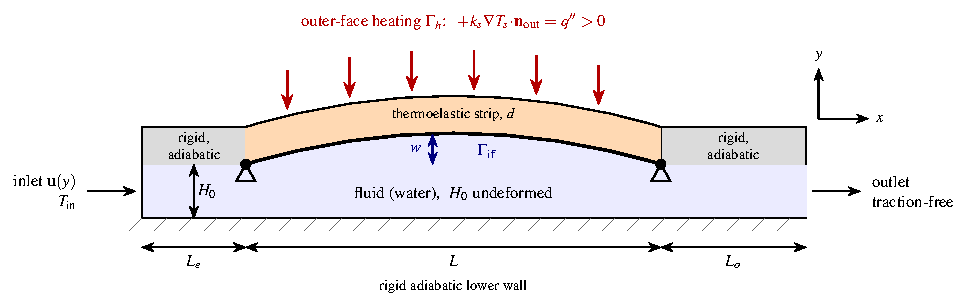
\includegraphics[width=\textwidth]{figures/fig1_geometry.pdf}
\caption{Configuration (schematic, not to scale; the strip thickness and the bow are exaggerated).
A thermoelastic strip of length $L$ and thickness $d$ forms part of the upper wall of a slit
channel of undeformed height $H_0$. The outer face $\Ga_h$ receives a prescribed heat flux $\qpp>0$
into the strip. With pinned ends the strip bows away from the channel: the interface deflection
$w$ is positive away from the channel and the passage widens.}
\label{fig:geometry}
\end{figure}

\begin{table}[t]
\centering\small
\caption{Geometry and operating point of the baseline (design values).}
\label{tab:geometry}
\begin{tabular}{@{}llll@{}}
\toprule
Quantity & Symbol & Value & Note \\
\midrule
Undeformed channel height & $H_0$ & \SI{0.50}{\milli\metre} & design input \\
Hydraulic diameter (slit) & $D_h=2H_0$ & \SI{1.0}{\milli\metre} & derived \\
Deformable (heated) length & $L$ & \SI{30}{\milli\metre} & design \\
Entrance / exit length & $L_e$, $L_o$ & \SI{10}{\milli\metre}, \SI{20}{\milli\metre} & design \\
Strip thickness & $d$ & \SI{3.0}{\milli\metre} & design \\
Mean inlet velocity & $U$ & \SI{0.050}{\metre\per\second} & design \\
Imposed outer-face heat flux & $\qpp$ & \SI{5.0}{\kilo\watt\per\square\metre} & design \\
\bottomrule
\end{tabular}
\end{table}

The following assumptions define the model; each is checked for the baseline in
Section~\ref{sec:baseline}.
\begin{description}[leftmargin=0pt,labelindent=0pt,style=unboxed,font=\normalfont\bfseries]
\item[A1] \emph{Plane strain.} The out-of-plane dimension is large compared with $H_0$ and $d$ and
the loading is uniform along it, so the fields are two-dimensional and $\varepsilon_{zz}=0$ in the
solid \citep{boley1960theory,timoshenko1970elasticity}.
\item[A2] \emph{Newtonian, constant-property water} at near-ambient temperature. Laminar, steady
flow ($\mathrm{Re}_{D_h}=\NumRe$); viscous dissipation and buoyancy are negligible at the baseline
(Section~\ref{sec:baseline}).
\item[A3] \emph{Homogeneous, isotropic, linearly thermoelastic solid} of constant $E$, $\nu$,
$\alpha$, $k_s$. The values are representative of an unfilled PEEK-class polymer
(Table~\ref{tab:props}); they are not frozen against a specific datasheet, and every derived number
scales with them.
\item[A4] \emph{Small strains and moderate rotations}, with the wall equation carried to the
von K\'arm\'an beam--column level of Section~\ref{sec:beamcolumn}.
\item[A5] \emph{Steady flow and energy, quasi-static solid.} The structural wave-crossing time of the
strip, $d\sqrt{\rho_s/E}\approx\SI{1.8}{\micro\second}$, is many orders of magnitude shorter than the
transport times, so inertia is omitted.
\item[A6] \emph{Perfect thermal contact} at $\Ga_{\mathrm{if}}$: temperature and normal heat flux are
continuous; no contact resistance.
\item[A7] \emph{Ideal pinned ends.} At $X=0,L$ the vertical displacement vanishes, the mean axial
displacement over the end edge vanishes, the applied moment is zero, and the heat flux is zero. This
is a pin and not a clamp: a clamp forbids end rotation, and a clamped strip at uniform curvature
does not bow at all (Section~\ref{sec:freecurv}).
\item[A8] \emph{Idealised heater.} The heater is represented only by a uniform flux $\qpp$ entering
the solid through $\Ga_h$. Heater construction, heater--wall contact resistance and heat loss from
the outer face are not modelled; all of $\qpp$ is assumed to enter the strip.
\item[A9] \emph{Rigid casing as a support, not as a contact.} The casing fixes the end conditions and
the reference pressure of the cavity above the strip (equal to the outlet datum). The model contains
no contact between the deformed strip and the casing and no casing clearance; the cavity above the
strip is assumed to leave room for the computed deflection.
\end{description}

\subsection{Governing equations}
\label{sec:governing}
\emph{Fluid.} On the deformed fluid domain $\Om_f$ (Section~\ref{sec:ale}), steady incompressible
flow with constant properties obeys, in the standard form \citep{bird1960transport},
\begin{align}
\nabla\!\cdot\bu&=0, \label{eq:cont}\\
\rho\,(\bu\!\cdot\!\nabla)\bu&=-\nabla p+\mu\nabla^2\bu, \label{eq:mom}\\
\rho c_p\,(\bu\!\cdot\!\nabla)T_f&=k_f\nabla^2T_f. \label{eq:fe}
\end{align}
\emph{Solid.} On the reference configuration $\Om_s^0$ steady conduction \citep{carslaw1947conduction}
and linear thermoelastic equilibrium without inertia hold,
\begin{align}
\nabla\!\cdot(k_s\nabla T_s)&=0, \label{eq:cond}\\
\nabla\!\cdot\bsig=\bm 0,\qquad
\bsig&=2\mu_L\beps+\lambda(\operatorname{tr}\beps)\bI-\beta\theta\bI,\qquad
\beps=\tfrac12\!\left(\nabla\bd+\nabla\bd^{\mathsf T}\right), \label{eq:solid}
\end{align}
with $\theta=T_s-T_{\mathrm{ref}}$, Lam\'e parameters $\lambda,\mu_L$ and thermoelastic pressure
coefficient $\beta=E\alpha/(1-2\nu)$ \citep{boley1960theory}. In plane strain the out-of-plane
stress is $\sigma_{zz}=\nu(\sigma_{xx}+\sigma_{yy})-E\alpha\theta$ and is part of the stress state; all
stresses reported below are total Cauchy stresses. The deformation-heating source of the transient
thermoelastic energy equation vanishes identically in a steady state, so \eqref{eq:cond} is exact
for the steady problem.

\emph{Reduced wall equation.} For design estimates the strip is treated as an Euler--Bernoulli strip
of flexural rigidity per unit depth $D_s=Ed^3/[12(1-\nu^2)]$, the wide-strip value appropriate to plane strain,
\begin{equation}
D_s\,w^{\prime\prime\prime\prime}=p(x),\qquad w(0)=w(L)=w^{\prime\prime}(0)=w^{\prime\prime}(L)=0,
\label{eq:beam}
\end{equation}
where $p$ is the fluid pressure acting on the strip (positive pushes the strip away from the channel).
This equation is used for estimates and benchmarks only; the two-dimensional system
\eqref{eq:cond}--\eqref{eq:solid} is the model.

\subsection{Deformed domain}
\label{sec:ale}
The fluid problem is posed on the domain occupied by the fluid in the converged steady state. Given
the solid displacement on $\Ga_{\mathrm{if}}^0$, a mesh displacement $\bwhat$ is obtained on
$\Om_f^0$ from a pseudo-elastic extension problem with $\bwhat=\bd$ on $\Ga_{\mathrm{if}}^0$ and
$\bwhat=\bm 0$ on rigid boundaries, and $\Om_f=\{X+\bwhat(X)\}$. No time derivative appears, so no mesh
velocity or geometric-conservation-law constraint arises in the steady problem
\citep{lesoinne1996geometric}.

\subsection{Sign conventions, interface and boundary conditions}
\label{sec:bc}
A single unit normal $\bn$, pointing from the fluid into the solid, is used on $\Ga_{\mathrm{if}}$.
Pressure is positive in compression and stress is positive in tension. The coordinate $y$ points from
the fluid into the solid. The deflection $w$ is measured \emph{away from the channel},
$w=+d_2$ with $d_2$ the displacement in $+y$; the thermal curvature $\kth>0$ is the curvature that
bows the strip away from the channel, and within small slopes $\kappa=-w^{\prime\prime}$. The heat flux
vector is $\bm q=-k\nabla T$, and $\qpp>0$ denotes heat \emph{supplied} to the solid.

On the deformed interface the subsystems exchange kinematics, traction and heat:
\begin{align}
\bu&=\bm 0 && \text{(no slip, steady form of }\bu=\partial_t\bd), \label{eq:ifkin}\\
\bsig\bn&=\left(-p\bI+2\mu\bD(\bu)\right)\bn && \text{(traction continuity)}, \label{eq:iftrac}\\
T_f&=T_s && \text{(temperature continuity)}, \label{eq:iftemp}\\
-k_f\nabla T_f\!\cdot\!\bn&=-k_s\nabla T_s\!\cdot\!\bn && \text{(normal heat-flux continuity)}, \label{eq:ifflux}
\end{align}
with $\bD(\bu)=\tfrac12(\nabla\bu+\nabla\bu^{\mathsf T})$. The exterior conditions are listed in
Table~\ref{tab:bcs}. Condition B5 makes the sign of the thermal load explicit: with the outward
normal $\bn_{\mathrm{out}}=+\bm e_y$ of the solid on $\Ga_h$, the flux $\bm q\cdot\bn_{\mathrm{out}}=-k_s\partial_yT_s$
equals $-\qpp$ (inward), so $k_s\,\partial_yT_s=+\qpp>0$: the temperature rises towards the outer
face, which is therefore the hot face.

\begin{table}[t]
\centering\small
\caption{Boundary conditions. $\bn_{\mathrm{out}}$ is the outward normal of the solid.}
\label{tab:bcs}
\begin{tabular}{@{}p{0.7cm}p{3.2cm}p{9.2cm}@{}}
\toprule
ID & Boundary & Condition \\
\midrule
B1 & inlet $x=-L_e$ & $\bu=6U\frac{y}{H_0}\left(1-\frac{y}{H_0}\right)\bm e_x$, $T_f=T_{\mathrm{in}}$ \\
B2 & outlet $x=L+L_o$ & traction-free (do-nothing) outflow, $\partial_nT_f=0$ \\
B3 & lower wall $y=0$ & $\bu=\bm 0$, $\partial_nT_f=0$ (rigid, adiabatic) \\
B4 & rigid casing sections & $\bu=\bm 0$, $\partial_nT_f=0$ \\
B5 & outer face $\Ga_h^0$ & $+k_s\nabla T_s\!\cdot\!\bn_{\mathrm{out}}=\qpp$ with $\qpp>0$ heat supplied to the solid \\
B6 & strip ends $X=0,L$ & $d_2=0$, $\langle d_1\rangle=0$ (edge mean), zero applied moment, $\partial_nT_s=0$ \\
B7 & remaining solid faces & zero traction, zero heat flux \\
B8 & interface $\Ga_{\mathrm{if}}$ & \eqref{eq:ifkin}--\eqref{eq:ifflux} \\
\bottomrule
\end{tabular}
\end{table}

\subsection{Material data}
\label{sec:props}
Table~\ref{tab:props} lists the properties. Water values are standard near-ambient data. The solid
values are representative of unfilled PEEK and are datasheet-representative, not grade-specific.

\begin{table}[t]
\centering\small
\caption{Material properties used in all calculations.}
\label{tab:props}
\begin{tabular}{@{}llll@{}}
\toprule
Property & Symbol & Value & Unit \\
\midrule
Water density, viscosity & $\rho$, $\mu$ & $1.0\times10^{3}$, $1.0\times10^{-3}$ & \si{\kilo\gram\per\cubic\metre}, \si{\pascal\second} \\
Water specific heat, conductivity & $c_p$, $k_f$ & $4.18\times10^{3}$, $0.60$ & \si{\joule\per\kilo\gram\per\kelvin}, \si{\watt\per\metre\per\kelvin} \\
Solid Young's modulus, Poisson ratio & $E$, $\nu$ & $3.6\times10^{9}$, $0.40$ & \si{\pascal}, -- \\
Solid expansion coefficient & $\alpha$ & $5.0\times10^{-5}$ & \si{\per\kelvin} \\
Solid conductivity & $k_s$ & $0.25$ & \si{\watt\per\metre\per\kelvin} \\
Solid yield stress (guard only) & $\sigma_y$ & $9\times10^{7}$ & \si{\pascal} \\
\bottomrule
\end{tabular}
\end{table}

\section{Reduced-order thermoelastic analysis of the strip}
\label{sec:reduced}

This section derives the closed-form relations used to size the deformation before any coupled
computation. All of them follow from the model of Section~\ref{sec:formulation} under the stated
assumptions; the numerical values at the baseline are collected in Section~\ref{sec:baseline}.

\subsection{Free thermal curvature and the sign chain}
\label{sec:freecurv}
Let $\eta$ be the coordinate across the strip measured from the mid-plane (positive towards the outer
face), and let the temperature be linear,
$\theta(\eta)=\bar\theta+\Gamma\eta$, with $\Gamma=\Delta T_t/d>0$ by condition B5. For a thin strip with
traction-free faces $\sigma_{yy}\simeq0$, and plane strain gives
$\sigma_{xx}=E'[\varepsilon_{xx}-(1+\nu)\alpha\theta]$ with $E'=E/(1-\nu^2)$. With
$\varepsilon_{xx}=\varepsilon_0+\kappa\eta$, a vanishing axial force resultant gives
$\varepsilon_0=(1+\nu)\alpha\bar\theta$, and a vanishing moment resultant gives the free thermal
eigen-curvature
\begin{equation}
\kth=(1+\nu)\,\alpha\,\frac{\Delta T_t}{d}=(1+\nu)\,\alpha\,\frac{\qpp}{k_s},
\qquad \Delta T_t=\frac{\qpp d}{k_s}, \label{eq:kappa}
\end{equation}
where the second form uses one-dimensional steady conduction across the strip
\citep{carslaw1947conduction} and is the plane-strain form of the classical result
\citep{boley1960theory}. Two consequences follow. First, $\kth$ does not depend on $d$: the
through-thickness gradient adjusts to cancel the thickness. Second, a strip clamped at both ends
carries the constant restoring moment $D_s\kth$ and does not bow ($w\equiv0$); the bowing
mechanism exists only for pinned ends or for an axially non-uniform $\kth(x)$, which fixes the
support choice A7.

The sign chain is, in order: (i) $\qpp>0$ supplies heat to the outer face (B5); (ii) the temperature
therefore rises towards the outer face ($\Gamma>0$), which is the hot face; (iii) the hot fibres
elongate more, so the strip curves with the outer face convex, $\kth>0$; (iv) with pinned ends this
is an arch whose mid-span moves \emph{away} from the channel, $w>0$; (v) the passage height
$H=H_0+w$ increases. The same chain read backwards shows that a bow \emph{into} the passage
would require heating the fluid-facing face, which is a different model (Section~\ref{sec:limits}).

\subsection{Pinned bowing at negligible axial force}
\label{sec:pinned}
With $w^{\prime\prime}=-\kth$ and $w(0)=w(L)=0$,
\begin{equation}
w(x)=\frac{\kth}{2}\,x(L-x),\qquad \wmax^{\mathrm{lin}}=\frac{\kth L^2}{8}.
\label{eq:wlin}
\end{equation}
This is exact within thin-strip theory when the axial force is negligible, which is the state of a
strip free to expand axially.

\subsection{Thermal membrane force and buckling}
\label{sec:buckling}
With the axial displacement blocked at both ends the mean axial strain vanishes, and integration
across the thickness gives the compressive membrane force per unit depth
\begin{equation}
N_\theta=-\frac{E\,d\,\alpha\bar\theta}{1-\nu},\qquad \Nc=|N_\theta|. \label{eq:ntheta}
\end{equation}
The pinned--pinned Euler load of the wide strip is $\ncr=\pi^2D_s/L^2$ \citep{timoshenko1961stability}.
The wide-strip rigidity is the consistent one because plane strain suppresses the anticlastic
curvature mode. Setting $\Nc=\ncr$ gives the critical mean temperature rise
\begin{equation}
\bar T_{\mathrm{cr}}=\frac{\pi^2d^2}{12\,\alpha(1+\nu)L^2},\qquad
M_b=\frac{\bar T_{\mathrm{cr}}}{\bar\theta}, \label{eq:tcr}
\end{equation}
where the buckling margin $M_b$ is used as a guard. The mean wall rise is estimated as
$\bar\theta=\Delta T_t/2+\qpp/h+\Delta T_b/2$: half the through-wall drop, the interface excess over
the local bulk temperature with the rigid-slit coefficient $h=\mathrm{Nu}_{H1}k_f/D_h$ for one heated
wall \citep{shah1978laminar}, and half the bulk rise $\Delta T_b=\qpp L/(\rho UH_0c_p)$.

\subsection{Beam--column bowing at finite membrane force}
\label{sec:beamcolumn}
A pinned strip carrying the compressive force $\Nc$ couples its deflection to that force at leading
order. Retaining the geometric stiffness of the membrane force and freezing the force at its
blocked-state value, the transverse equilibrium of the strip, with total moment $M=D_s(w^{\prime\prime}+\kth)$
vanishing at the pins, is
\begin{equation}
D_s\,w^{\prime\prime\prime\prime}+\Nc\,w^{\prime\prime}=0,\qquad w(0)=w(L)=0,\quad
w^{\prime\prime}(0)=w^{\prime\prime}(L)=-\kth. \label{eq:beamcol}
\end{equation}
With $\mu^2=\Nc/D_s$ the solution is
\begin{equation}
w(x)=\frac{\kth}{\mu^2}\left[\frac{1-\cos\mu L}{\sin\mu L}\sin\mu x+\cos\mu x-1\right],\qquad
\wmax=\frac{\kth}{\mu^2}\left[\sec\frac{\mu L}{2}-1\right], \label{eq:wbc}
\end{equation}
which reduces to \eqref{eq:wlin} as $\mu L\to0$ and diverges at $\mu L=\pi$, the Euler threshold
\eqref{eq:tcr}: the bowing law and the buckling limit are two limits of one relation. The force
is not in fact frozen. With both ends blocked, the mean axial strain contains the arc-stretching
term $\tfrac12\langle w^{\prime2}\rangle$, so the signed force acquires the correction
\begin{equation}
N_\theta(w)=N_\theta+\frac{Ed}{2(1-\nu^2)}\,\langle w^{\prime2}\rangle,\qquad
\Nc^{\mathrm{sc}}=|N_\theta|-\frac{Ed}{2(1-\nu^2)}\langle w^{\prime2}\rangle, \label{eq:nupdate}
\end{equation}
which relaxes the compression. Because the family \eqref{eq:wbc} holds for every fixed force,
\eqref{eq:nupdate} is a scalar fixed-point problem for $\Nc^{\mathrm{sc}}$.

Two deflections are therefore defined, and they answer different questions. The \emph{frozen-force}
value $\wmax$ of \eqref{eq:wbc} with $\Nc=|N_\theta|$ is the exact solution of the stated
equation \eqref{eq:beamcol}; because it neglects the relaxation it overestimates the deflection and
is a conservative upper bound. The \emph{self-consistent} value solves \eqref{eq:wbc} with
$\Nc^{\mathrm{sc}}$ and is the von K\'arm\'an equilibrium of the reduced strip. It is also what the
coupled algorithm of Section~\ref{sec:algorithm} converges to, since it re-evaluates the membrane force at
every iteration. The self-consistent value is therefore quoted as the model's best estimate, and the
frozen-force value as the upper bound; both are reported. The two differ by \NumExcessFrozen\,\% at
the baseline, \NumExcessW\,\% and \NumExcessS\,\% at the heat fluxes of guards G1 and G2
(Section~\ref{sec:guards}), and \NumExcessB\,\% at $\Nc/\ncr=0.5$, where the frozen-force form should
no longer be used.

\subsection{Hydraulic loading and the thermal-to-hydraulic ratio}
\label{sec:hydraulic}
Integrating plane Poiseuille flow \citep{bird1960transport,shah1978laminar} gives the slit pressure
drop
\begin{equation}
\Delta p=\frac{12\mu UL}{H_0^2}. \label{eq:dp}
\end{equation}
With the outlet datum $p=0$ and the casing cavity at the same reference pressure (A9), the gauge
pressure on the strip falls linearly from $p(0)=p(L)+\Delta p$ at its upstream end to
$p(L)=12\mu UL_o/H_0^2$ at its downstream end, with mean $\bar p=\tfrac12[p(0)+p(L)]$. For pinned ends, a uniform load
$\bar p$ acting in the same sense as the thermal bow deflects the strip by
$w_p=5\bar pL^4/(384D_s)$ at the linear level \citep{timoshenko1970elasticity}; the mild variation of
the load is neglected in this estimate. The ratio of the thermal to the hydraulic deflection of the
\emph{same} strip is
\begin{equation}
\Gamma_p=\frac{w_{\mathrm{th}}}{w_p},\qquad
\Gamma_p^{\mathrm{lin}}=\frac{\wmax^{\mathrm{lin}}}{w_p}=\frac{48\,\kth D_s}{5\,\bar pL^2}, \label{eq:gammap}
\end{equation}
where $\Gamma_p^{\mathrm{lin}}$ uses both deflections at zero membrane force. A second like-for-like
form, $\Gamma_p^{\Nc}$, computes both deflections with the same compressive force $\Nc$: the thermal
deflection from \eqref{eq:wbc} and the pressure deflection from the beam--column equation
$D_sw^{\prime\prime\prime\prime}+\Nc w^{\prime\prime}=\bar p$. Both forms compare two responses of one
structure in one state and are therefore directly comparable. A ratio that places the thermal
deflection \emph{with} the beam--column amplification over a pressure deflection \emph{without} it
mixes two states of the structure and is not used. Because $\kth$ is independent of $d$ while
$D_s\propto d^3$ and $\bar p\propto UH_0^{-2}$, $\Gamma_p$ grows with wall thickness and falls with
velocity and with decreasing channel height.

\subsection{Admissibility guards}
\label{sec:guards}
Five guards bound the regime in which the reduced-order model and the weak form of
Section~\ref{sec:fe} are used. (G1) $\wmax/H_0\le0.5$, so that the deformed fluid mesh keeps positive
Jacobians. (G2) $\sigma_{\max}\le0.2\,\sigma_y$, with $\sigma_{\max}$ the sum of the bending stress
$6|M_{\mathrm{mid}}|/d^2$ at mid-span and the membrane stress $E\alpha\bar\theta/(1-\nu)$.
(G3) $M_b\ge2$. (G4) $\Gamma_p\ge5$, the threshold above which the thermal bow is the dominant
deformation. (G5) $\mathrm{Re}_{D_h}\le100$, $\mathrm{Br}<10^{-2}$ and a Richardson number small enough
for the neglect of buoyancy, with $\mathrm{Ri}=g\beta_f\Delta T^{*}H_0/U^2$ and $\Delta T^{*}=\qpp H_0/k_f$.

\section{Baseline results of the reduced-order model}
\label{sec:baseline}

All values in this section are computed by the program \texttt{code/hff\_model.py} from the inputs of
Tables~\ref{tab:geometry} and~\ref{tab:props} and the relations of Section~\ref{sec:reduced};
Table~\ref{tab:baseline} collects them. Quantities that depend on the solid properties scale with
the datasheet values, which are not frozen (A3).

\begin{table}[t]
\centering\small
\caption{Reduced-order baseline at the design point of Table~\ref{tab:geometry}. The deflection and
passage height are given for the self-consistent state (sc) and, as an upper bound, for the
frozen-force state (ff).}
\label{tab:baseline}
\begin{tabular}{@{}p{4.4cm}p{4.6cm}p{4.9cm}@{}}
\toprule
Quantity & Expression & Value \\
\midrule
Reynolds, P\'eclet numbers & $2\rho UH_0/\mu$; $\mathrm{Re}\,\mathrm{Pr}$ & $\NumRe$; $\NumPe$ (Pr $=\NumPr$) \\
Rigid-slit pressure drop & $12\mu UL/H_0^2$ \eqref{eq:dp} & \SI{\NumDp}{\pascal}; wall shear \SI{\NumTauW}{\pascal} \\
Through-wall temperature drop & $\Delta T_t=\qpp d/k_s$ & \SI{\NumDTt}{\kelvin} \\
Bulk rise; interface excess & $\Delta T_b$; $\qpp/h$ with $h=\NumHrigid\,\si{\watt\per\square\metre\per\kelvin}$ & \SI{\NumDTb}{\kelvin}; \SI{\NumQoverH}{\kelvin} \\
Mean wall temperature rise & $\bar\theta=\Delta T_t/2+\qpp/h+\Delta T_b/2$ & \SI{\NumThetaBar}{\kelvin} \\
Free thermal curvature & $(1+\nu)\alpha\qpp/k_s$ \eqref{eq:kappa} & \SI{\NumKappa}{\per\metre} \\
Linear bow & $\kth L^2/8$ \eqref{eq:wlin} & $\NumWlin$~m $=\NumWlinH\,H_0$ \\
Membrane force; Euler load & $N_c$ \eqref{eq:ntheta}; $\ncr=\pi^2D_s/L^2$ & $\NumNtheta$; $\NumNcr$ N\,m$^{-1}$; $N_c/\ncr=\NumNratio$ \\
Critical rise; buckling margin & $\bar T_{\mathrm{cr}}$; $M_b$ \eqref{eq:tcr} & \SI{\NumTcr}{\kelvin}; $\NumMb$ \\
Beam--column parameter & $\mu L=L\sqrt{N_c/D_s}$ & $\NumMuL$ \\
Bow, frozen force (ff) & \eqref{eq:wbc} & $\NumWfrozen$~m $=\NumWfrozenH\,H_0$ \\
Bow, self-consistent (sc) & \eqref{eq:wbc}, \eqref{eq:nupdate} & $\NumWsc$~m $=\NumWscH\,H_0$ \\
Mid-span passage height $H_0+\wmax$ & derived & $\NumHmidSc\,H_0$ (sc); $\NumHmidFrozen\,H_0$ $=$ \SI{\NumHmidMm}{\milli\metre} (ff) \\
Slope, strains (ff) & $\max|w^\prime|$; $\tfrac12\langle w^{\prime2}\rangle$; bending fibre strain & $\NumSlope$; $\NumArcStrain$; $\NumFibreStrain$ \\
Stresses (ff) & bending; membrane; sum & \SI{\NumSigBend}{\mega\pascal}; \SI{\NumSigMemb}{\mega\pascal}; \SI{\NumSigMax}{\mega\pascal} $=\NumSigFrac\,\sigma_y$ \\
Gauge pressure on the strip & $p(0)$; $p(L)$; $\bar p$ & \SI{\NumPentry}{\pascal}; \SI{\NumPexit}{\pascal}; \SI{\NumPbar}{\pascal} \\
Hydraulic deflection & $5\bar pL^4/(384D_s)$ & $\NumWp$~m (zero force); $\NumWpBC$~m (with $N_c$) \\
Thermal-to-hydraulic ratio & $\Gamma_p^{\mathrm{lin}}$; $\Gamma_p^{N_c}$ \eqref{eq:gammap} & $\NumGammaLinRound$; $\NumGammaBCRound$ \\
Buoyancy, dissipation & $\mathrm{Ri}$; $\mathrm{Br}$ & $\NumRi$; $\NumBr$ \\
\bottomrule
\end{tabular}
\end{table}

\subsection{Deformation of the passage}
\label{sec:deform}
The strip bows away from the channel by $\wmax=\NumWsc$~m, which is $\NumWscH\,H_0$, in the
self-consistent state; the frozen-force upper bound is $\NumWfrozenH\,H_0$
(Figure~\ref{fig:bowing}a). The passage height at mid-span is $H=H_0+\wmax=\NumHmidSc\,H_0$
(sc) or $\NumHmidFrozen\,H_0$ (ff), that is \SI{\NumHmidMm}{\milli\metre} against the undeformed
\SI{0.50}{\milli\metre}. This is a \emph{derived beam-model passage height}, not a prescribed
clearance: it is the sum of the design height $H_0$ and the computed deflection, and nothing in the
model constrains it from above (assumption A9). A two-dimensional finite-element solution of the restrained wall (Section~\ref{sec:q8nl}) gives
$\NLwFEH\,H_0$, $\NLoverScPct\,\%$ above the self-consistent value.
The beam--column amplification over the linear bow
is $\NumAmpFrozen$, consistent at leading order with the Euler factor $1/(1-N_c/\ncr)=\NumAmpEuler$.
The strains and the slope are small ($\max|w^\prime|=\NumSlope$, bending fibre strain
$\NumFibreStrain$), which supports the small-strain, moderate-rotation level of A4.

\begin{figure}[t]
\centering
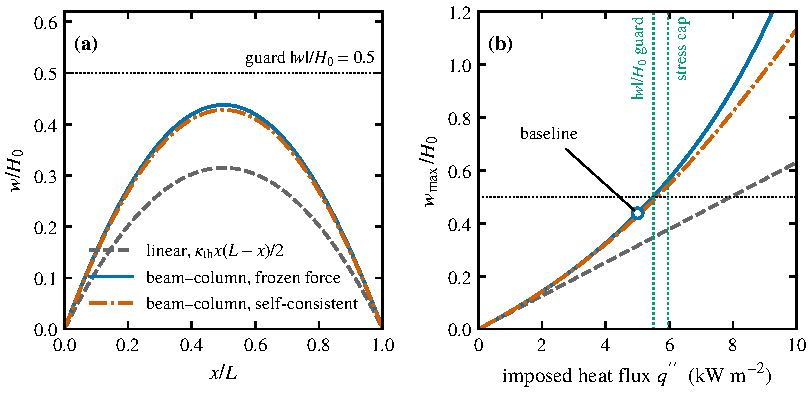
\includegraphics[width=\textwidth]{figures/fig2_bowing.pdf}
\caption{Bowing of the strip (positive away from the channel). (a) Deflection profile at the
baseline: linear estimate \eqref{eq:wlin}, frozen-force beam--column \eqref{eq:wbc} and
self-consistent beam--column \eqref{eq:wbc}--\eqref{eq:nupdate}. (b) Mid-span deflection against the
imposed flux; vertical dotted lines mark the fluxes at which guards G1 ($|w|/H_0=0.5$) and G2
(stress cap) are reached. The marker is the baseline.}
\label{fig:bowing}
\end{figure}

\subsection{Guards and heat-flux ceilings}
\label{sec:ceilings}
The baseline lies inside all five guards of Section~\ref{sec:guards}: $\wmax/H_0=\NumWfrozenH$ (ff)
against 0.5; $\sigma_{\max}=\NumSigFrac\,\sigma_y$ against 0.2; $M_b=\NumMb$ against 2;
$\Gamma_p=\NumGammaLinRound$ against 5; $\mathrm{Re}_{D_h}=\NumRe$, $\mathrm{Br}=\NumBr$ and
$\mathrm{Ri}=\NumRi$. All but the last are exceeded in the order deformation, stress, buckling as
$\qpp$ increases, because $\kth$ and $\bar\theta$ both scale with $\qpp$. In the frozen-force state G1
is reached at $\qpp=\SI{\NumQw}{\kilo\watt\per\square\metre}$ ($N_c/\ncr=\NumRatioW$), G2 at
\SI{\NumQs}{\kilo\watt\per\square\metre} ($\wmax/H_0=\NumWHs$), and the buckling margin $M_b=2$ at
\SI{\NumQb}{\kilo\watt\per\square\metre}, where $\wmax/H_0=\NumWHb$ would long since be
unacceptable. The binding constraints are therefore deformation and stress, with buckling the outer
ceiling, and the baseline flux is already \SI{9}{\percent} below the first of them.

Buoyancy and viscous dissipation do not enter the baseline: $\mathrm{Ri}=\NumRi$ and $\mathrm{Br}=\NumBr$.
Stratification can destabilise horizontal flows when it is strong, as studied for a fluid with large
property variations by \citet{draskic2025stability}; that regime is not approached here.

The stress is dominated by the compressive membrane component, \SI{\NumSigMemb}{\mega\pascal}, a
by-product of the axial constraint that also produces the buckling limit; the bending component is
\SI{\NumSigBend}{\mega\pascal}.

\subsection{Role of the wall material}
Because $\kth=(1+\nu)\alpha\qpp/k_s$, the choice of wall material sets the size of the effect. For
typical austenitic stainless steel ($k_s\approx\SI{16}{\watt\per\metre\per\kelvin}$,
$\alpha\approx\SI{1.7e-5}{\per\kelvin}$, $\nu=0.30$) at the same flux and geometry,
$\kth=\NumStainlessKappa$~\si{\per\metre} and $\wmax^{\mathrm{lin}}/H_0=\NumStainlessWH$: about
$\NumPolymerOverStainless$ times smaller than for the polymer, a physically real deformation but
irrelevant to the convective field. The combination of low conductivity and high expansion
coefficient of the polymer class, not any fluid-side property, selects the design space.

\subsection{Indicative consequences for the flow}
\label{sec:indicative}
The deformation is large enough to change the passage substantially, so two flow-side consequences
are estimated. Both are reduced-order and indicative only; the coupled computation is required to
quantify them. \emph{Hydraulic.} With the flow rate per unit depth $UH_0$ fixed and the local height
$H(x)=H_0+w(x)$, the lubrication estimate is
$\Delta p=12\mu UH_0\int_0^L\dd x/H^3$, which is $\NumDpLub$~Pa, a factor $\NumDpLubRatio$ of the
rigid-slit value \eqref{eq:dp}, a drop of about $\NumDpLubDrop$ per cent (Figure~\ref{fig:passage}b).
The lubrication parameter $\mathrm{Re}_{H_0}H_0/L=\NumReHL$ is not small, so the value indicates that the
hydraulic effect is of order one rather than giving its magnitude. \emph{Thermal.} With a
quasi-developed local coefficient $h(x)=\mathrm{Nu}_{H1}k_f/[2H(x)]$ the mean interface excess
$\qpp/h$ rises from \SI{\NumQoverH}{\kelvin} to \SI{\NumExcessDeformed}{\kelvin} (a factor
$\NumExcessRatio$). The thermal entry length is about \SI{\NumLT}{\milli\metre}, so $L/L_T=\NumLoverLT$
and the quasi-developed assumption is not justified; this too is an order-of-magnitude indicator.

\begin{figure}[t]
\centering
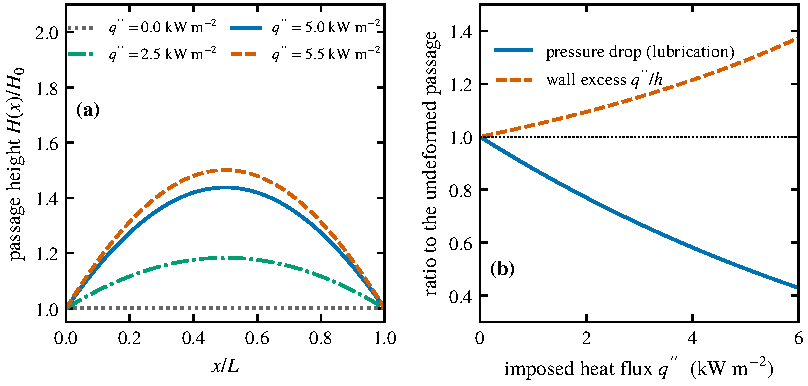
\includegraphics[width=\textwidth]{figures/fig3_passage.pdf}
\caption{Reduced-order consequences of the deformation (indicative). (a) Passage height $H(x)/H_0$
for several imposed fluxes (frozen-force bow). (b) Lubrication estimate of the pressure drop and
quasi-developed estimate of the mean interface excess $\qpp/h$, both relative to the undeformed
passage.}
\label{fig:passage}
\end{figure}

\emph{Feedback onto the deflection.} The larger interface excess raises $\bar\theta$ by about
\SI{\NumFeedbackExtraK}{\kelvin} out of \SI{\NumThetaBar}{\kelvin}, which increases $\wmax$ by only
\NumFeedbackPct\,\%; the hydraulic load changes the deflection by $\NumHydFeedbackPct$\,\% of the
thermal bow ($1/\Gamma_p$). At the baseline the effect of the wall on the flow is therefore large,
whereas the effect of the flow back on the wall is small, because $\kth$ depends on $\qpp$ and on the wall
properties only (equation~\eqref{eq:kappa}) and the thermal loop enters through $\bar\theta$ alone.
Whether the closed loop matters elsewhere in the parameter space is a question for the coupled
computation, not for this reduced-order model.

\section{Finite-element formulation and verification}
\label{sec:fem}

This section specifies the finite-element method for the coupled problem of Section~\ref{sec:formulation},
states what has and has not been verified, and reports the verification of the wall idealisation.
\textbf{The coupled fluid--structure--thermal solver is specified here but no result of it is reported.}
The only finite-element computations in this paper are those of the wall in
Section~\ref{sec:q8}.

\subsection{Discretisation}
\label{sec:fe}
\emph{Meshes.} The fluid and the solid are meshed separately but conformingly: the two meshes share the
nodes of $\Ga_{\mathrm{if}}$, so that interface data need no interpolation. The fluid mesh follows the
deformed interface through the extension problem of Section~\ref{sec:ale}.

\emph{Fluid.} Velocity and pressure use the Taylor--Hood pair, continuous quadratic velocity and
continuous linear pressure (P2--P1), which satisfies the discrete inf--sup condition
\citep{hood1974navier,brezzi1991mixed}. On $\Om_f$ the weak form seeks $(\bu,p)$ with $\bu$ satisfying B1
and B3--B4 and the interface condition $\bu=\bm0$ such that, for all admissible $(\bv,q)$,
\begin{equation}
\int_{\Om_f}\!\left[\rho(\bu\!\cdot\!\nabla\bu)\!\cdot\!\bv+2\mu\,\bD(\bu)\!:\!\bD(\bv)-p\,\nabla\!\cdot\!\bv+q\,\nabla\!\cdot\!\bu\right]\dd\Om=0,
\label{eq:wkfluid}
\end{equation}
where the do-nothing outflow B2 is the natural condition. The convective term is linearised by Newton
iteration.

\emph{Energy.} Temperature is one continuous quadratic field $T$ on $\Om_f\cup\Om_s$ with the
conductivity $k=k_f$ or $k_s$ and the velocity $\bu$ in the fluid and zero in the solid. Because the
meshes are conforming, temperature continuity \eqref{eq:iftemp} is enforced strongly and the flux
continuity \eqref{eq:ifflux} is the natural interface condition: there is a \emph{single} interface
temperature unknown and no thermal interface iteration. With B5 the weak form is
\begin{equation}
\int_{\Om_f\cup\Om_s}\!\left[\rho c_p(\bu\!\cdot\!\nabla T)\,\phi+k\,\nabla T\!\cdot\!\nabla\phi\right]\dd\Om
+\sum_K\int_K\tau_K\,\rho c_p\,\bu\!\cdot\!\nabla\phi\,\mathcal R_K(T)\,\dd\Om=\int_{\Ga_h}\qpp\,\phi\,\dd\Ga,
\label{eq:wkenergy}
\end{equation}
with the element residual $\mathcal R_K(T)=\rho c_p\,\bu\!\cdot\!\nabla T-k_f\nabla^2T$. The
streamline-upwind/Petrov--Galerkin (SUPG) term \citep{brooks1982streamline} is required: the P\'eclet number is
$\mathrm{Pe}=\NumPe$, so that a Galerkin discretisation without stabilisation is expected to oscillate on any mesh whose
streamwise spacing is not of micrometre order. The stabilisation parameter is
$\tau_K=\tfrac{h_K}{2|\bu|_K}\left(\coth\mathrm{Pe}_K-1/\mathrm{Pe}_K\right)$ with
$\mathrm{Pe}_K=\rho c_p|\bu|_Kh_K/(2k_f)$ and $\tau_K=0$ in the solid.

\emph{Solid.} The displacement is continuous quadratic. To retain the beam--column amplification of
Section~\ref{sec:beamcolumn} the solid is solved in a total-Lagrangian description with the
Green--Lagrange strain $\bm E=\tfrac12(\bm F^{\mathsf T}\bm F-\bm I)$, the deformation gradient
$\bm F=\bm I+\nabla\bd$, and the St~Venant--Kirchhoff law with the in-plane thermal eigenstrain of A1,
\begin{equation}
\bm S=\mathbb C\!:\!\left[\bm E-(1+\nu)\alpha\,\theta\,\bm I\right],\qquad
\int_{\Om_s^0}\bm S\!:\!\delta\bm E\,\dd\Om=\int_{\Ga_{\mathrm{if}}^0}\bm t\!\cdot\!\delta\bd\,\dd\Ga,
\label{eq:wksolid}
\end{equation}
where, for small strain and rotation, \eqref{eq:wksolid} reduces to the linear system \eqref{eq:solid}, and $\theta=T_s-T_{\mathrm{in}}$ is the temperature rise and $\bm t$ is the fluid traction pulled back to
the reference interface. The tangent of \eqref{eq:wksolid} contains a material part and a geometric part
that carries the thermal membrane stress; the latter is what produces the amplification
$1/(1-N_c/\ncr)$. A linear solid omits it (Section~\ref{sec:q8nl}).

\subsection{Coupled fixed-point algorithm}
\label{sec:algorithm}
The mechanical coupling is a Dirichlet--Neumann partition: the fluid receives the interface displacement
through the mesh extension, and the solid receives the interface traction. With the thermal problem
solved as one field, the outer iteration $k=0,1,\dots$ on the deformed geometry
$\Om^k$ ($\Om^0$ undeformed) is:
\begin{enumerate}
\item solve the Navier--Stokes problem \eqref{eq:wkfluid} on $\Om_f^k$ for $(\bu^k,p^k)$ and form the
interface traction $\bm t^k$;
\item solve the energy problem \eqref{eq:wkenergy} on $\Om_f^k\cup\Om_s^k$ for $T^k$, hence $\theta^k$ in the solid;
\item solve \eqref{eq:wksolid} with $\theta^k$ and $\bm t^k$ for $\bd^{k+1}$;
\item relax, $\bd^{k+1}\leftarrow\omega\bd^{k+1}+(1-\omega)\bd^k$ with $0<\omega\le1$ (Aitken updating is optional), and
update the fluid mesh through the extension problem of Section~\ref{sec:ale};
\item stop when $\|\bd^{k+1}-\bd^k\|/\|\bd^{k+1}\|$ and the relative interface heat-flux imbalance are below tolerances.
\end{enumerate}
The guards of Section~\ref{sec:guards} are monitored during the iteration; in particular the
mesh-quality guard G1 keeps the extension problem well posed. A partitioned thermal alternative, in which
the interface temperature is imposed as a Dirichlet condition on the solid and the flux as a Neumann
condition on the fluid, is possible on the same meshes but is not needed here. \emph{No proof of convergence
of the fixed point is offered.} The reduced-order estimates of Section~\ref{sec:indicative} indicate a weak
return coupling at the baseline, which suggests contraction, but this has not been tested.

\subsection{Verification hierarchy}
\label{sec:hier}
Table~\ref{tab:hier} lists the verification levels needed before coupled results could be trusted and
shows which have been executed. Only the first four concern the wall and the reduced-order model; all
levels involving the fluid are planned.

\begin{table}[t]
\centering\small
\caption{Verification hierarchy. ``Done'' marks computations reported in this paper.}
\label{tab:hier}
\begin{tabular}{@{}p{0.8cm}p{6.4cm}p{4.6cm}p{1.3cm}@{}}
\toprule
Level & Test & Reference & Status \\
\midrule
V1 & Shape functions, patch test (Q8) & exact polynomial field & Done \\
V2 & Closed forms of Section~\ref{sec:reduced} against an independent boundary-value solution & analytic/numerical BVP & Done \\
V3 & Free bow of the wall, end supports, mesh study & $\kth L^2/8$ & Done \\
V4 & Restrained nonlinear wall, amplification and membrane force; independent code; thin-strip limit & beam--column & Done \\
V5 & Rigid slit, pressure drop and velocity profile & $12\mu UL/H_0^2$ (Poiseuille) & Planned \\
V6 & Rigid slit, one wall heated, developed Nusselt number & \citet{shah1978laminar} & Planned \\
V7 & Conjugate transfer with a rigid thick wall & \citet{rahimi2024conjugate} & Planned \\
V8 & Pressure-loaded compliant channel, flow rate--pressure drop & \citet{christov2018flow} & Planned \\
V9 & Mesh convergence of the coupled outputs ($w$, $\Delta p$, $\mathrm{Nu}$) & \citet{celik2008procedure} & Planned \\
V10 & Iteration history and interface energy balance of the fixed point & internal consistency & Planned \\
\bottomrule
\end{tabular}
\end{table}

\subsection{Verification of the wall idealisation}
\label{sec:q8}
Two plane-strain computations with eight-node serendipity (Q8) elements, $3\times3$ Gauss quadrature and
a sparse direct solver, are reported. Both are own implementations (\texttt{code/q8\_strip.py} and
\texttt{code/q8\_nonlinear.py}); the second is cross-checked with an independent code in Section~\ref{sec:slender}. The shape functions are checked for partition of unity and for their
derivatives against central differences, and the patch test (the exact stress-free thermal-bending field must
satisfy the discrete equations) is passed on every mesh with a maximum relative residual of
$\QPatchMax$.

\subsubsection{Free bow and end supports}
\label{sec:q8free}
With a linear through-thickness temperature of zero mean the beam theory gives the bow
$w=\kth L^2/8$ at mid-span (Section~\ref{sec:freecurv}). The finite-element value is sampled at the
\emph{fixed} physical point $(L/2,\,y=d/2)$ on every mesh, because a sampling height that changes with the
through-thickness refinement is not a property of the mesh. Three end idealisations are compared:
an ideal point pin ($u_y=0$ at the single mid-surface node of each end edge), the pin of the paper realised
as $u_y=0$ on the whole end edge, and a clamp ($u_x=u_y=0$ on the whole edge). Meshes range from $6\times2$ to
$192\times8$ elements ($N_x\times N_y$, at most \QElemMax{} elements); the results are normalised by
$\kth L^2/8$ and are in Table~\ref{tab:q8mesh} and Figure~\ref{fig:q8mesh}.

\begin{table}[t]
\centering\scriptsize
\caption{Free-bow study: mid-span, mid-surface deflection normalised by $\kth L^2/8$. The order $p$,
the extrapolated value and the grid-convergence index (GCI, safety factor 1.25) of the clamp are from the
last three axial refinements, $N_x=48,96,192$ \citep{celik2008procedure}.}
\label{tab:q8mesh}
% AUTO-GENERATED by make_numbers.py
\begin{tabular}{@{}rrcccccrr@{}}
\toprule
$N_y$ & elements & point pin & full-edge pin & clamp & clamp & $p$ & clamp, extrap. & GCI (\%) \\
 & ($N_x=192$) & ($N_x=192$) & ($N_x=192$) & ($N_x=24$) & ($N_x=192$) & & & \\
\midrule
2 & 384 & 1.00000 & 0.99793 & $-$0.0288 & $-$0.0195 & 1.7 & $-$0.0192 & 2.0 \\
4 & 768 & 1.00000 & 0.99800 & $-$0.0253 & $-$0.0180 & 1.3 & $-$0.0175 & 3.8 \\
8 & 1536 & 1.00000 & 0.99800 & $-$0.0238 & $-$0.0174 & 1.1 & $-$0.0168 & 4.2 \\
\bottomrule
\end{tabular}

\end{table}

\begin{figure}[t]
\centering
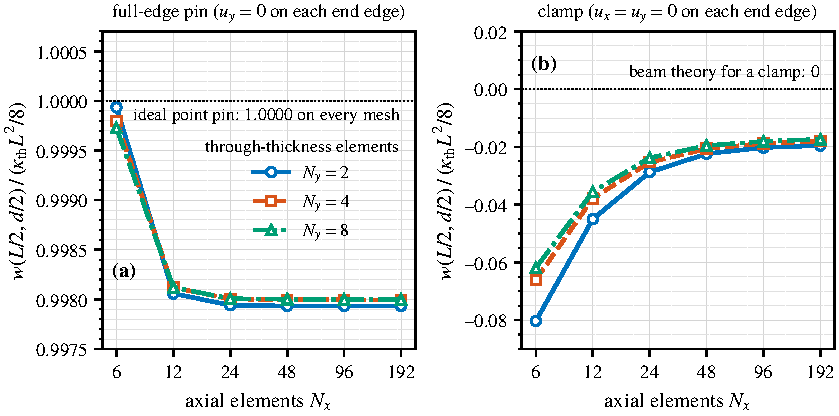
\includegraphics[width=\textwidth]{figures/fig4_q8_mesh.pdf}
\caption{Free-bow study against axial refinement $N_x$ for $N_y=2,4,8$ elements through the thickness.
(a) Pin realised as $u_y=0$ on each end edge. (b) Clamp.}
\label{fig:q8mesh}
\end{figure}

The ideal point pin returns $\QPointMin$ on every mesh, as it must: the exact field lies in the element
space, so this result tests the implementation and not the convergence. The pin of the paper, $u_y=0$ on the
whole edge, gives $\QPinFour$ at $192\times4$ and $\QPinEight$ at $192\times8$, a defect of
$\QPinDefect\,\%$. This is mesh-independent: the value changes by $\QPinAxialLast$ between $N_x=96$ and
$192$ at $N_y=8$ and by $\QPinThickLast$ between $N_y=4$ and $8$ at $N_x=192$. The defect is therefore a property of the
end condition and not a discretisation error. The clamp bows slightly \emph{towards} the channel. Beam theory
gives zero, since a clamp forbids end rotation and a uniform-curvature strip then does not bow; the
finite-element value converges slowly to a small negative number (Table~\ref{tab:q8mesh},
extrapolated $\QClampInfEight$ at $N_y=8$). The observed order is below two ($p=\QClampOrderEight$ at $N_y=8$), so the
asymptotic range has not been established and the GCI of $\QClampGCIEight\,\%$ is indicative only. The relevant
conclusions are that the pin idealisation is reproduced to $\QPinDefect\,\%$ and that the clamp, which is not
used in this paper, reduces the bow to $\QClampLastEight$ times the pinned bow, in agreement with beam theory (zero)
to that level.

\subsubsection{Restrained, geometrically nonlinear wall}
\label{sec:q8nl}
The baseline wall is not free: its ends are restrained axially (A7, B6), and the mean temperature rise
$\bar\theta=\NLthetaBar$~K produces the compressive membrane force $N_c$ of Section~\ref{sec:buckling}. The
second computation solves this problem: $\theta(Y)=\bar\theta+\Delta T_t(Y/d-\tfrac12)$ with the values of
Table~\ref{tab:baseline}, $u_y=0$ on the end edges, and a linear constraint that makes the mean axial displacement of each
end edge zero, eliminated exactly. The solid is the total-Lagrangian model \eqref{eq:wksolid} without
fluid load, solved by Newton iteration in four thermal load steps. The analytic tangent agrees with a central
finite difference of the residual to $\NLtangentMax$, and every step converged in at most $\NLnewtonMax$
iterations to a relative residual of $\NLresMax$. The same data are solved with the linear solid (material stiffness only)
for comparison; Table~\ref{tab:q8nl} and Figure~\ref{fig:q8nl} show the results.

\begin{table}[t]
\centering\small
\caption{Restrained wall at the baseline: linear and nonlinear Q8 solutions. $w^{\mathrm{lin}}$ is the
linear-solid mid-span deflection; $w_{\max}^{\mathrm{NL}}$ the total-Lagrangian one; $N_c$ is the
membrane force in the two element columns adjacent to mid-span.}
\label{tab:q8nl}
% AUTO-GENERATED by make_numbers.py
\begin{tabular}{@{}lrcccc@{}}
\toprule
mesh $N_x\times N_y$ & elements & $w^{\rm lin}/(\kth L^2/8)$ & $w_{\max}^{\rm NL}$ (\si{\micro\metre}) & $w_{\max}^{\rm NL}/H_0$ & $N_c$ at mid-span (kN\,m$^{-1}$) \\
\midrule
$24\times2$ & 48 & 0.9979 & 223.39 & 0.4468 & 27.79 \\
$48\times4$ & 192 & 0.9980 & 222.46 & 0.4449 & 27.74 \\
$96\times4$ & 384 & 0.9980 & 222.33 & 0.4447 & 27.74 \\
$96\times8$ & 768 & 0.9980 & 222.17 & 0.4443 & 27.73 \\
$192\times8$ & 1536 & 0.9980 & 222.14 & 0.4443 & 27.73 \\
\bottomrule
\end{tabular}

\end{table}

\begin{figure}[t]
\centering
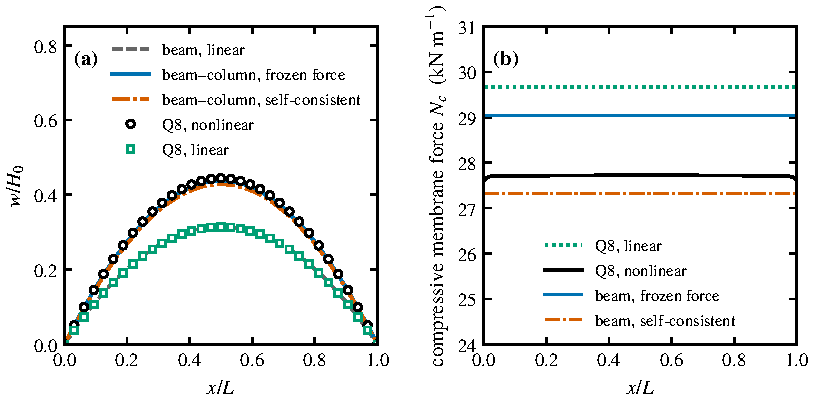
\includegraphics[width=\textwidth]{figures/fig5_q8_nonlinear.pdf}
\caption{Restrained baseline wall, finest mesh ($192\times8$). (a) Mid-surface deflection. (b) Compressive membrane
force per element column. Beam values are those of Table~\ref{tab:baseline}.}
\label{fig:q8nl}
\end{figure}

The results are as follows. (i) The linear-solid bow is $\NLlinRatio\,\kth L^2/8$, equal to the full-edge pin value of
Section~\ref{sec:q8free}: in a linear solid the membrane force does not couple to the bending. (ii) The
linear solution carries the membrane force $\NLNmidLin$~kN\,m$^{-1}$ at mid-span, $\NLNmidLinPct\,\%$ above the
frozen-force beam value of Table~\ref{tab:baseline}. (iii) The nonlinear solid bows by
$\NLwFE$~m ($\NLwFEH\,H_0$), an amplification $\NLampFE$ over the linear value, compared with $\NumAmpFrozen$
(frozen force) and $\NumAmpSc$ (self-consistent) in the beam--column model. A linear finite-element solid
therefore under-predicts the bow by a factor $\NLampFE$, which is why the total-Lagrangian form is specified in
Section~\ref{sec:fe}. (iv) The membrane force relaxes from $\NLNmidLin$ to $\NLNmidNL$~kN\,m$^{-1}$, that is by
$\NLrelaxFE\,\%$, against $\NumRelax\,\%$ in the beam model: the arc-stretching relaxation of
Section~\ref{sec:beamcolumn} is reproduced in magnitude. (v) The finite-element deflection exceeds the
self-consistent beam--column value by $\NLoverScPct\,\%$ and the frozen-force value by $\NLoverFrozenPct\,\%$.
(vi) The nonlinear result changes by $\NLconvAxial\,\%$ between $N_x=96$ and $192$ and by $\NLconvThick\,\%$ between
$N_y=4$ and $8$, so it is mesh-converged at this level.

\subsubsection{Independent solution and the thin-strip limit}
\label{sec:slender}
\emph{Independent code.} The same boundary-value problem was solved with a different code base and discretisation:
scikit-fem, six-node quadratic triangles, Lagrange-multiplier constraints for the end conditions, a different mesh
(\IndElements{} triangles at the finest level) and different quadrature (\texttt{code/fe\_independent.py}). It gives
$\IndW$~m for the nonlinear bow, which differs from the Q8 value by $\IndDiffPct\,\%$, and the mid-span membrane force
differs by $\IndNDiffPct\,\%$; the linear solutions agree to within $10^{-4}\,\%$. The result of the triangle mesh
itself changes by $\IndConv\,\%$ between the last two refinements. The two codes share the equations
(St~Venant--Kirchhoff kinematics, eigenstrain model), so this agreement verifies the implementation and the
discretisation but not the modelling assumptions.

\emph{Is the departure from the beam model a thickness effect?} Beam theory contains neither shear flexibility nor
end effects, so if the $\NLoverScPct\,\%$ of item (v) were due to the thickness of the strip ($d/L=0.1$) it must
vanish as $d/L\to0$ at fixed dimensionless loading. The study of Table~\ref{tab:slender} keeps the free curvature and the
force ratio $N_c/\ncr=\SlForceRatio$ fixed (so $\bar\theta\propto d^2$ and $\Delta T_t\propto d$) and varies $d$ with the
independent code. The departure from the self-consistent beam--column value falls from $\SlFirstPct\,\%$ at $d/L=0.1$ to
$\SlMidPct\,\%$ at $d/L=\SlMidDL$ and $\SlLastPct\,\%$ at $d/L=\SlLastDL$, roughly as $(d/L)^2$, and the
finite-element membrane force tends to the self-consistent beam force. At $d/L=\SlLastDL$ the result changes by only $\SlMeshPct\,\%$ between the $192\times8$ and $384\times16$ meshes, so the
residual of $\SlLastPct\,\%$ is not a mesh error. It is of the size expected of the higher-order rotation terms that the
von K\'arm\'an beam--column model omits (the maximum slope is $\NumSlope$), but this was not isolated. The departure of the baseline is therefore a finite-thickness effect of the
two-dimensional wall, and not a disagreement between the equations of the beam model and those of the finite-element
model. The finite-element value, in contrast, lies $\SlLastFrozenPct\,\%$ below the frozen-force value at $d/L=\SlLastDL$: its proximity to the baseline
finite-element result ($\NLoverFrozenPct\,\%$) is a coincidence of thickness, not an accuracy property.

\begin{table}[t]
\centering\small
\caption{Thin-strip study with the independent code: curvature $\kth=\NumKappa$~m$^{-1}$ and $N_c/\ncr=\SlForceRatio$ held
fixed, mesh $192\times8$. Columns: linear bow relative to $\kth L^2/8$, nonlinear bow relative to the self-consistent (sc)
and frozen-force (ff) beam--column values, and membrane force relative to the self-consistent beam force.}
\label{tab:slender}
% AUTO-GENERATED by make_numbers.py
\begin{tabular}{@{}cccccc@{}}
\toprule
$d/L$ & $d$ (mm) & $w^{\rm lin}_{\rm FE}/w^{\rm lin}_{\rm beam}$ & $w^{\rm NL}_{\rm FE}/w_{\rm sc}$ & $w^{\rm NL}_{\rm FE}/w_{\rm ff}$ & $N_{c,\rm FE}/N_c^{\rm sc}$ \\
\midrule
0.100 & 3.00 & 0.9980 & 1.0383 & 1.0152 & 1.0146 \\
0.075 & 2.25 & 0.9989 & 1.0233 & 0.9846 & 1.0083 \\
0.050 & 1.50 & 0.9995 & 1.0092 & 0.9330 & 1.0021 \\
0.035 & 1.05 & 0.9998 & 1.0017 & 0.8720 & 0.9993 \\
0.025 & 0.75 & 0.9999 & 0.9976 & 0.7990 & 1.0010 \\
\bottomrule
\end{tabular}

\end{table}

For the baseline strip the reduced-order deflection of Section~\ref{sec:baseline} is therefore a slight under-estimate,
by $\NLoverScPct\,\%$, of the two-dimensional wall response. For design use the finite-element value
$\NLwFEH\,H_0$ should be preferred for this thickness; the guard values and ceiling heat fluxes derived from the
reduced-order model are correspondingly slightly non-conservative.

\subsection{What has been verified}
The reduced-order model of the wall is verified against an independent boundary-value solution (V2) and, in
two dimensions, against finite elements (two independent codes) for the free bow, the end condition, the membrane force and the
nonlinear amplification, including the limit of a slender strip (V1, V3, V4). The constitutive and kinematic assumptions common to all
the wall models are not independently validated against experiment. The fluid-side estimates of Section~\ref{sec:indicative}, the coupling
algorithm and the formulation of the interface remain unverified until V5--V10 are carried out.

\section{Conclusions and limitations}
\label{sec:conclusions}

A thin thermoelastic strip heated on its outer face bows \emph{away from the channel}: the through-wall
temperature difference sets a free curvature $\kth=(1+\nu)\alpha\qpp/k_s$ that is independent of the strip thickness,
and pinned ends turn it into a bow that widens the passage. At the baseline the reduced-order bow is
$\NumWscH\,H_0$ and a two-dimensional geometrically nonlinear finite-element solution of the wall gives
$\NLwFEH\,H_0$, which is $\NLoverScPct\,\%$ higher; the beam--column amplification of the free bow
($\NLampFE$ in the finite-element solution) and the relaxation of the membrane force
($\NLrelaxFE\,\%$ against $\NumRelax\,\%$) are both reproduced in magnitude. The binding limits on the heat flux are
deformation and stress, with buckling an outer ceiling. Indicative flow-side estimates, which need the coupled
computation for confirmation, point to a hydraulic effect of order one and a notable rise of the wall excess
temperature, while the effect of the flow back on the bow is small at the baseline.

The verification is partial. Only the wall has been verified (levels V1--V4 of Table~\ref{tab:hier}); the
fluid, the interface formulation and the coupled algorithm are specified and unverified (V5--V10).

\subsection*{Limitations}\label{sec:limits}
\begin{itemize}
\item \textbf{No coupled results.} Every flow-side number is a reduced-order estimate (Section~\ref{sec:indicative}),
and the lubrication and quasi-developed assumptions are not justified at the baseline parameters.
\item \textbf{Material data} are representative of an unfilled PEEK-class polymer and not frozen against a
datasheet; they are constant with temperature, and the strip is linearly thermoelastic (A3).
\item \textbf{Idealisations.} Perfect thermal contact (A6), ideal pinned ends (A7), an idealised uniform heater
(A8), and a casing that is only a support, with no contact with the deformed strip and no clearance (A9). A real
mounting would change the end conditions and, with them, the bow (Section~\ref{sec:q8free}).
\item \textbf{Heated face.} The model heats the outer face. Heating the fluid-facing face would bow the strip into the
channel and is a different model, outside this paper.
\item \textbf{Two dimensions.} Plane strain is assumed; end effects and finite thickness may explain part of the
finite-element departure from the beam model; shear flexibility accounts for a small share of it, and most of the
$\NLoverScPct\,\%$ has not been attributed.
\item \textbf{Steady state.} Transient heating, thermal inertia and viscoelasticity of the polymer are not
modelled.
\end{itemize}

\subsection*{Further work}
Carry out V5--V10 of Table~\ref{tab:hier}; compute the coupled problem and test the contraction of the
fixed point; replace the idealised heater and end conditions with a specified mounting and casing contact; and
validate against experiment.


\appendix
\section{Nomenclature}
\label{app:symbols}
\begin{table}[h]
\centering\small
\caption{Principal symbols (SI units).}
\label{tab:symbols}
\begin{tabular}{@{}p{2.0cm}p{5.1cm}p{2.0cm}p{5.1cm}@{}}
\toprule
Symbol & Meaning & Symbol & Meaning \\
\midrule
$H_0$ & undeformed passage height & $\kth$ & free thermal curvature \\
$L$, $d$ & strip length and thickness & $\nu$, $E$ & Poisson ratio, Young modulus \\
$L_e$, $L_o$ & entrance and outlet lengths & $\alpha$ & thermal expansion coefficient \\
$U$ & mean inlet velocity & $k_s$, $k_f$ & solid and fluid conductivity \\
$\qpp$ & imposed heat flux (supplied) & $D_s$ & flexural rigidity per unit depth \\
$\bu$, $p$ & velocity, pressure & $N_c$, $\ncr$ & compressive membrane force, Euler load \\
$T$, $\theta$ & temperature, rise above inlet & $M_b$ & buckling margin \\
$\bar\theta$ & mean wall temperature rise & $\wmax$ & maximum deflection (away from channel) \\
$\Delta T_t$, $\Delta T_b$ & through-wall and bulk temperature rise & $\Gamma_p$ & thermal-to-hydraulic deflection ratio \\
$\mathrm{Re}$, $\mathrm{Pr}$, $\mathrm{Pe}$ & Reynolds, Prandtl, P\'eclet numbers & $\mathrm{Ri}$, $\mathrm{Br}$ & Richardson, Brinkman numbers \\
$\bd$, $\bsig$, $\beps$ & displacement, stress, strain & $\bm F$, $\bm E$, $\bm S$ & deformation gradient, Green--Lagrange strain, second Piola--Kirchhoff stress \\
$\Ga_{\mathrm{if}}$, $\Ga_h$ & interface, heated outer face & $\bn$, $\bn_{\mathrm{out}}$ & interface normal, outward solid normal \\
\bottomrule
\end{tabular}
\end{table}


\bibliographystyle{emerald_harvard}
\bibliography{references}

\end{document}
